\documentclass{beamer}

\useoutertheme[subsection=false]{miniframes}
\usecolortheme{beaver}
\setbeamertemplate{navigation symbols}{}
\setbeamertemplate{footline}{}
\usepackage{graphicx}
\usepackage{url}
\usepackage{datetime}
\usepackage{tikz-cd}
\newcommand{\lectureDate}{\formatdate{20}{11}{2018}}

\setbeamertemplate{caption}
{\raggedright\insertcaption\par}
\title{MATH211: Linear Methods I}
\author{Matthew Burke}
\date{\lectureDate}
\begin{document}

\frame{\titlepage}

\begin{frame}{Lecture on \lectureDate}
  \tableofcontents
\end{frame}

\section*{Last time}
\label{sec:Last-time}

\begin{frame}{Summary of previous work}
\begin{itemize}
	\item $i^2=-1$
	\begin{itemize}
		\item $(a+bi)+(c+di) = (a+c)+(b+d)i$
		\item $(a+bi)(c+di) = (ac -bd)+(ad+bc)i$
	\end{itemize}\vfill
	\item graphical interpretation
	\begin{align*}
		a+bi &\leftrightarrow (a, b)\\
		\mathbb{C} &\leftrightarrow \mathbb{R}^2
	\end{align*}\vfill
	\item polar form
	\begin{equation*}
		a+ib \leftrightarrow Re^{i\theta}
	\end{equation*}
	where $R$ is the \emph{modulus} and $\theta$ the \emph{angle}.
\end{itemize}
\end{frame}

\section{Examples}

\begin{frame}{Examples}
\begin{example}
Convert the following to polar form:-
\begin{itemize}
	\item $-2+2\sqrt{3}i$ % ANS: 4e^{i*2*pi/3}
	\item $3i$ % ANS: 3e^{i*pi/2}
	\item $-1-i$ % ANS: sqrt{2}e^{i*5*pi/4}
	\item $\sqrt{3}+3i$ % ANS: 2*sqrt(3)e^{i*pi/3}
\end{itemize}
\end{example}
\begin{example}
Convert the following to standard form:-
\begin{itemize}
	\item $2e^{\frac{2\pi i}{3}}$ % ANS: -1+sqrt(3)i
	\item $3e^{-i\pi}$ % ANS: -3
	\item $2e^{\frac{3i\pi}{4}}$ % ANS: -sqrt{2}+sqrt{2}i
\end{itemize}
\end{example}
\end{frame}

\section{Multiplication}

\begin{frame}
\begin{beamercolorbox}[sep=12pt,center]{part title}
\usebeamerfont{section title}
\insertsection\par
\end{beamercolorbox}
\end{frame}

\begin{frame}{Multiplication using polar form}
If $z=Re^{i\theta}$ and $w=Qe^{i\phi}$ then
\begin{align*}
zw&=Re^{i\theta}Qe^{i\phi}\\
 &= (RQ)e^{i(\theta+\phi)}
\end{align*}\vfill
{\bf Slogan:} To multiply two complex numbers we multiply the moduli and add the angles.\vfill
\begin{theorem}[De Moivre Theorem]
	\begin{equation*}
	(\cos\theta+i\sin\theta)^n = (e^{i\theta})^n = e^{in\theta} = \cos(n\theta)+i\sin(n\theta)
	\end{equation*}
	\end{theorem}
\end{frame}

\begin{frame}{Questions?}
Questions?
\end{frame}

\begin{frame}{Examples}
\begin{example}
Express $(1-i)^6(\sqrt{3}+i)^3$ in the form $a+bi$. % ANS: -64
\end{example}
\begin{example}
Express $(\frac{1}{2}-\frac{\sqrt{3}}{2}i)^{17}$ in the form $a+bi$. % ANS: 1/2 + (sqrt{3}/2)i
\end{example}
\end{frame}

\section{Complex roots}

\begin{frame}
\begin{beamercolorbox}[sep=12pt,center]{part title}
\usebeamerfont{section title}
\insertsection\par
\end{beamercolorbox}
\end{frame}

\begin{frame}{Principal square roots}
Now we know that:\vfill
{\bf Slogan:} To multiply two complex numbers we multiply the moduli and add the angles.\vfill
So we could try reversing this:\vfill
{\bf Slogan:} To find the principal square root we take the square root of the modulus and halve the angle.\vfill
\begin{itemize}
	\item (The answer will depend on the angle measuring convention.)
\end{itemize}
\end{frame}

\begin{frame}{Picture}
If $z = e^{i\alpha}$ has unit modulus:\vfill
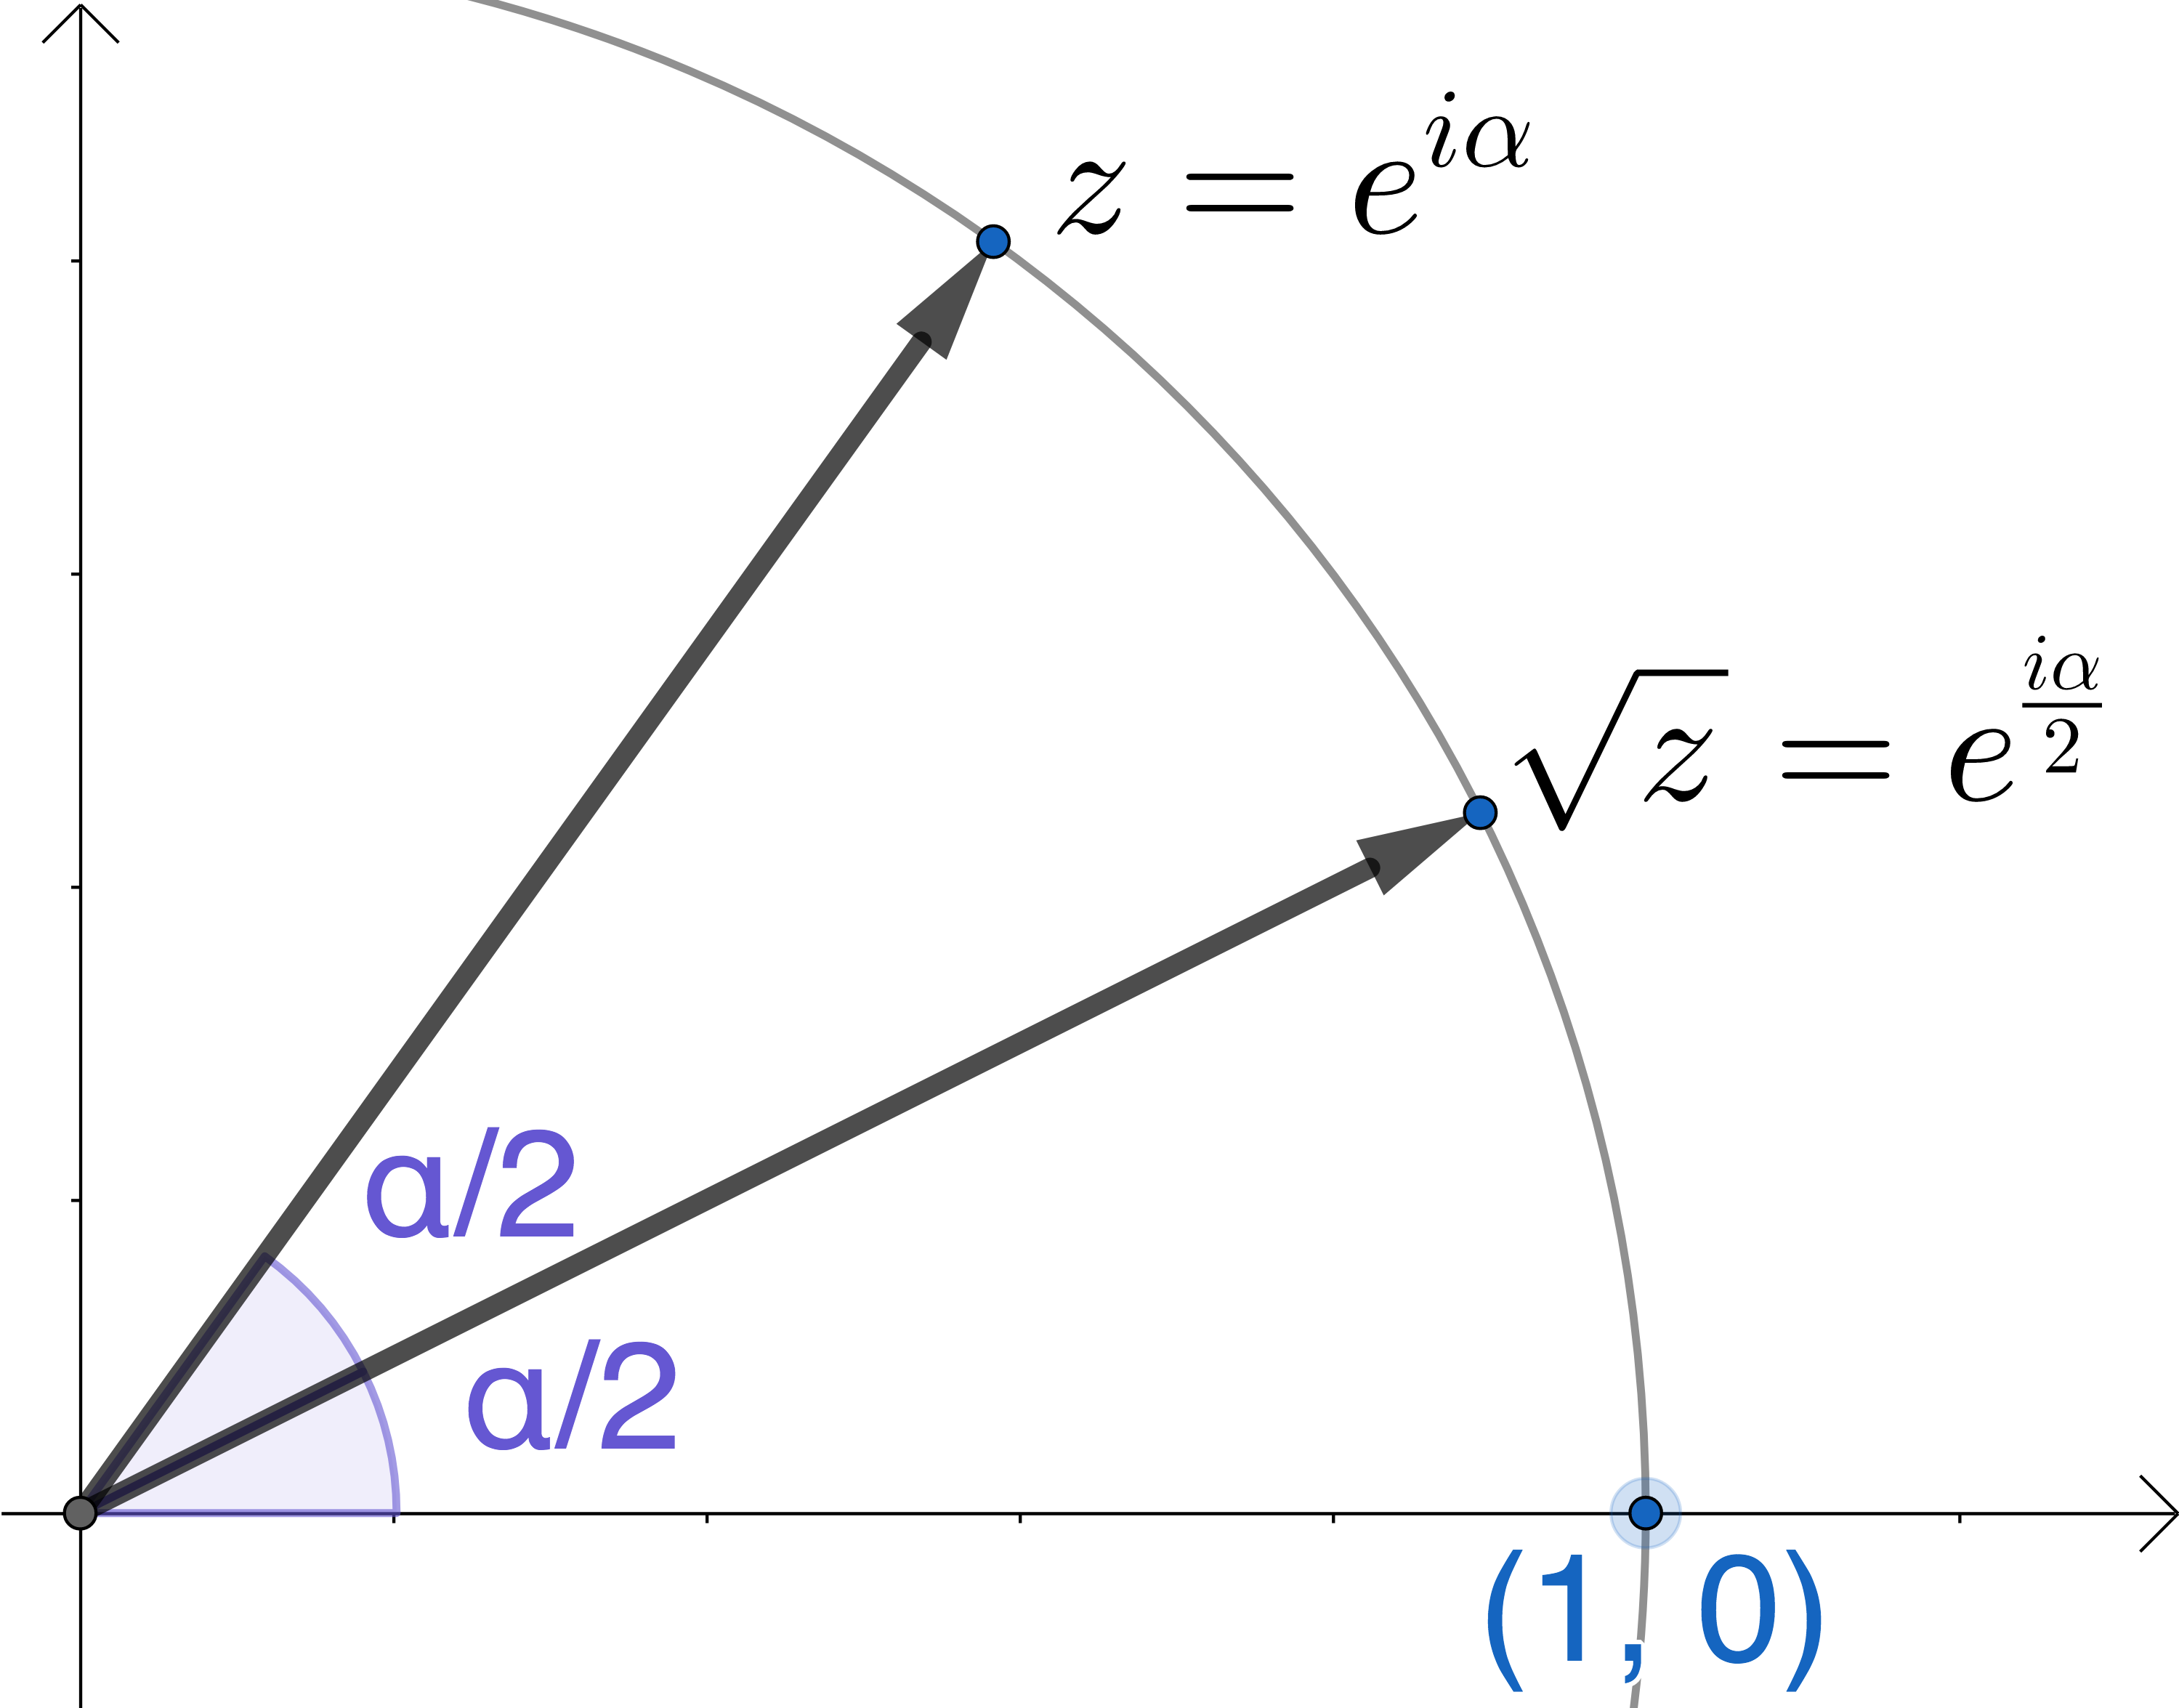
\includegraphics[scale=5]{principal-square-root.png}
\end{frame}

\begin{frame}{Non-principal square roots}
Let $z = R\cdot e^{i\alpha}$ and take the principal square root:\vfill
{\LARGE
\begin{equation*}
\sqrt{z} = \sqrt{R\cdot e^{i\alpha}} = \sqrt{R}\cdot e^{\frac{i\alpha}{2}}
\end{equation*}
}\vfill
Then all of numbers of the form\vfill
{\LARGE
\begin{equation*}
\sqrt{R}\cdot e^{(\frac{i\alpha}{2}+ki\cdot\pi)}
\end{equation*}
}\vfill
for $k\in \mathbb{Z}$ are \emph{also} a square roots of $z$:\vfill
{\LARGE
\begin{equation*}
\left(\sqrt{R}\cdot e^{(\frac{i\alpha}{2}+ki\pi)}\right)^2 = R\cdot e^{i\alpha + 2ki\pi} = R\cdot e^{i\alpha} = z
\end{equation*}
}
\end{frame}

\begin{frame}{Example}
  	The two square roots of $z = e^{\frac{i\pi}{4}}$ are $e^{\frac{i\pi}{8}}$ and $e^{\frac{-7i\pi}{8}}$:\vfill
	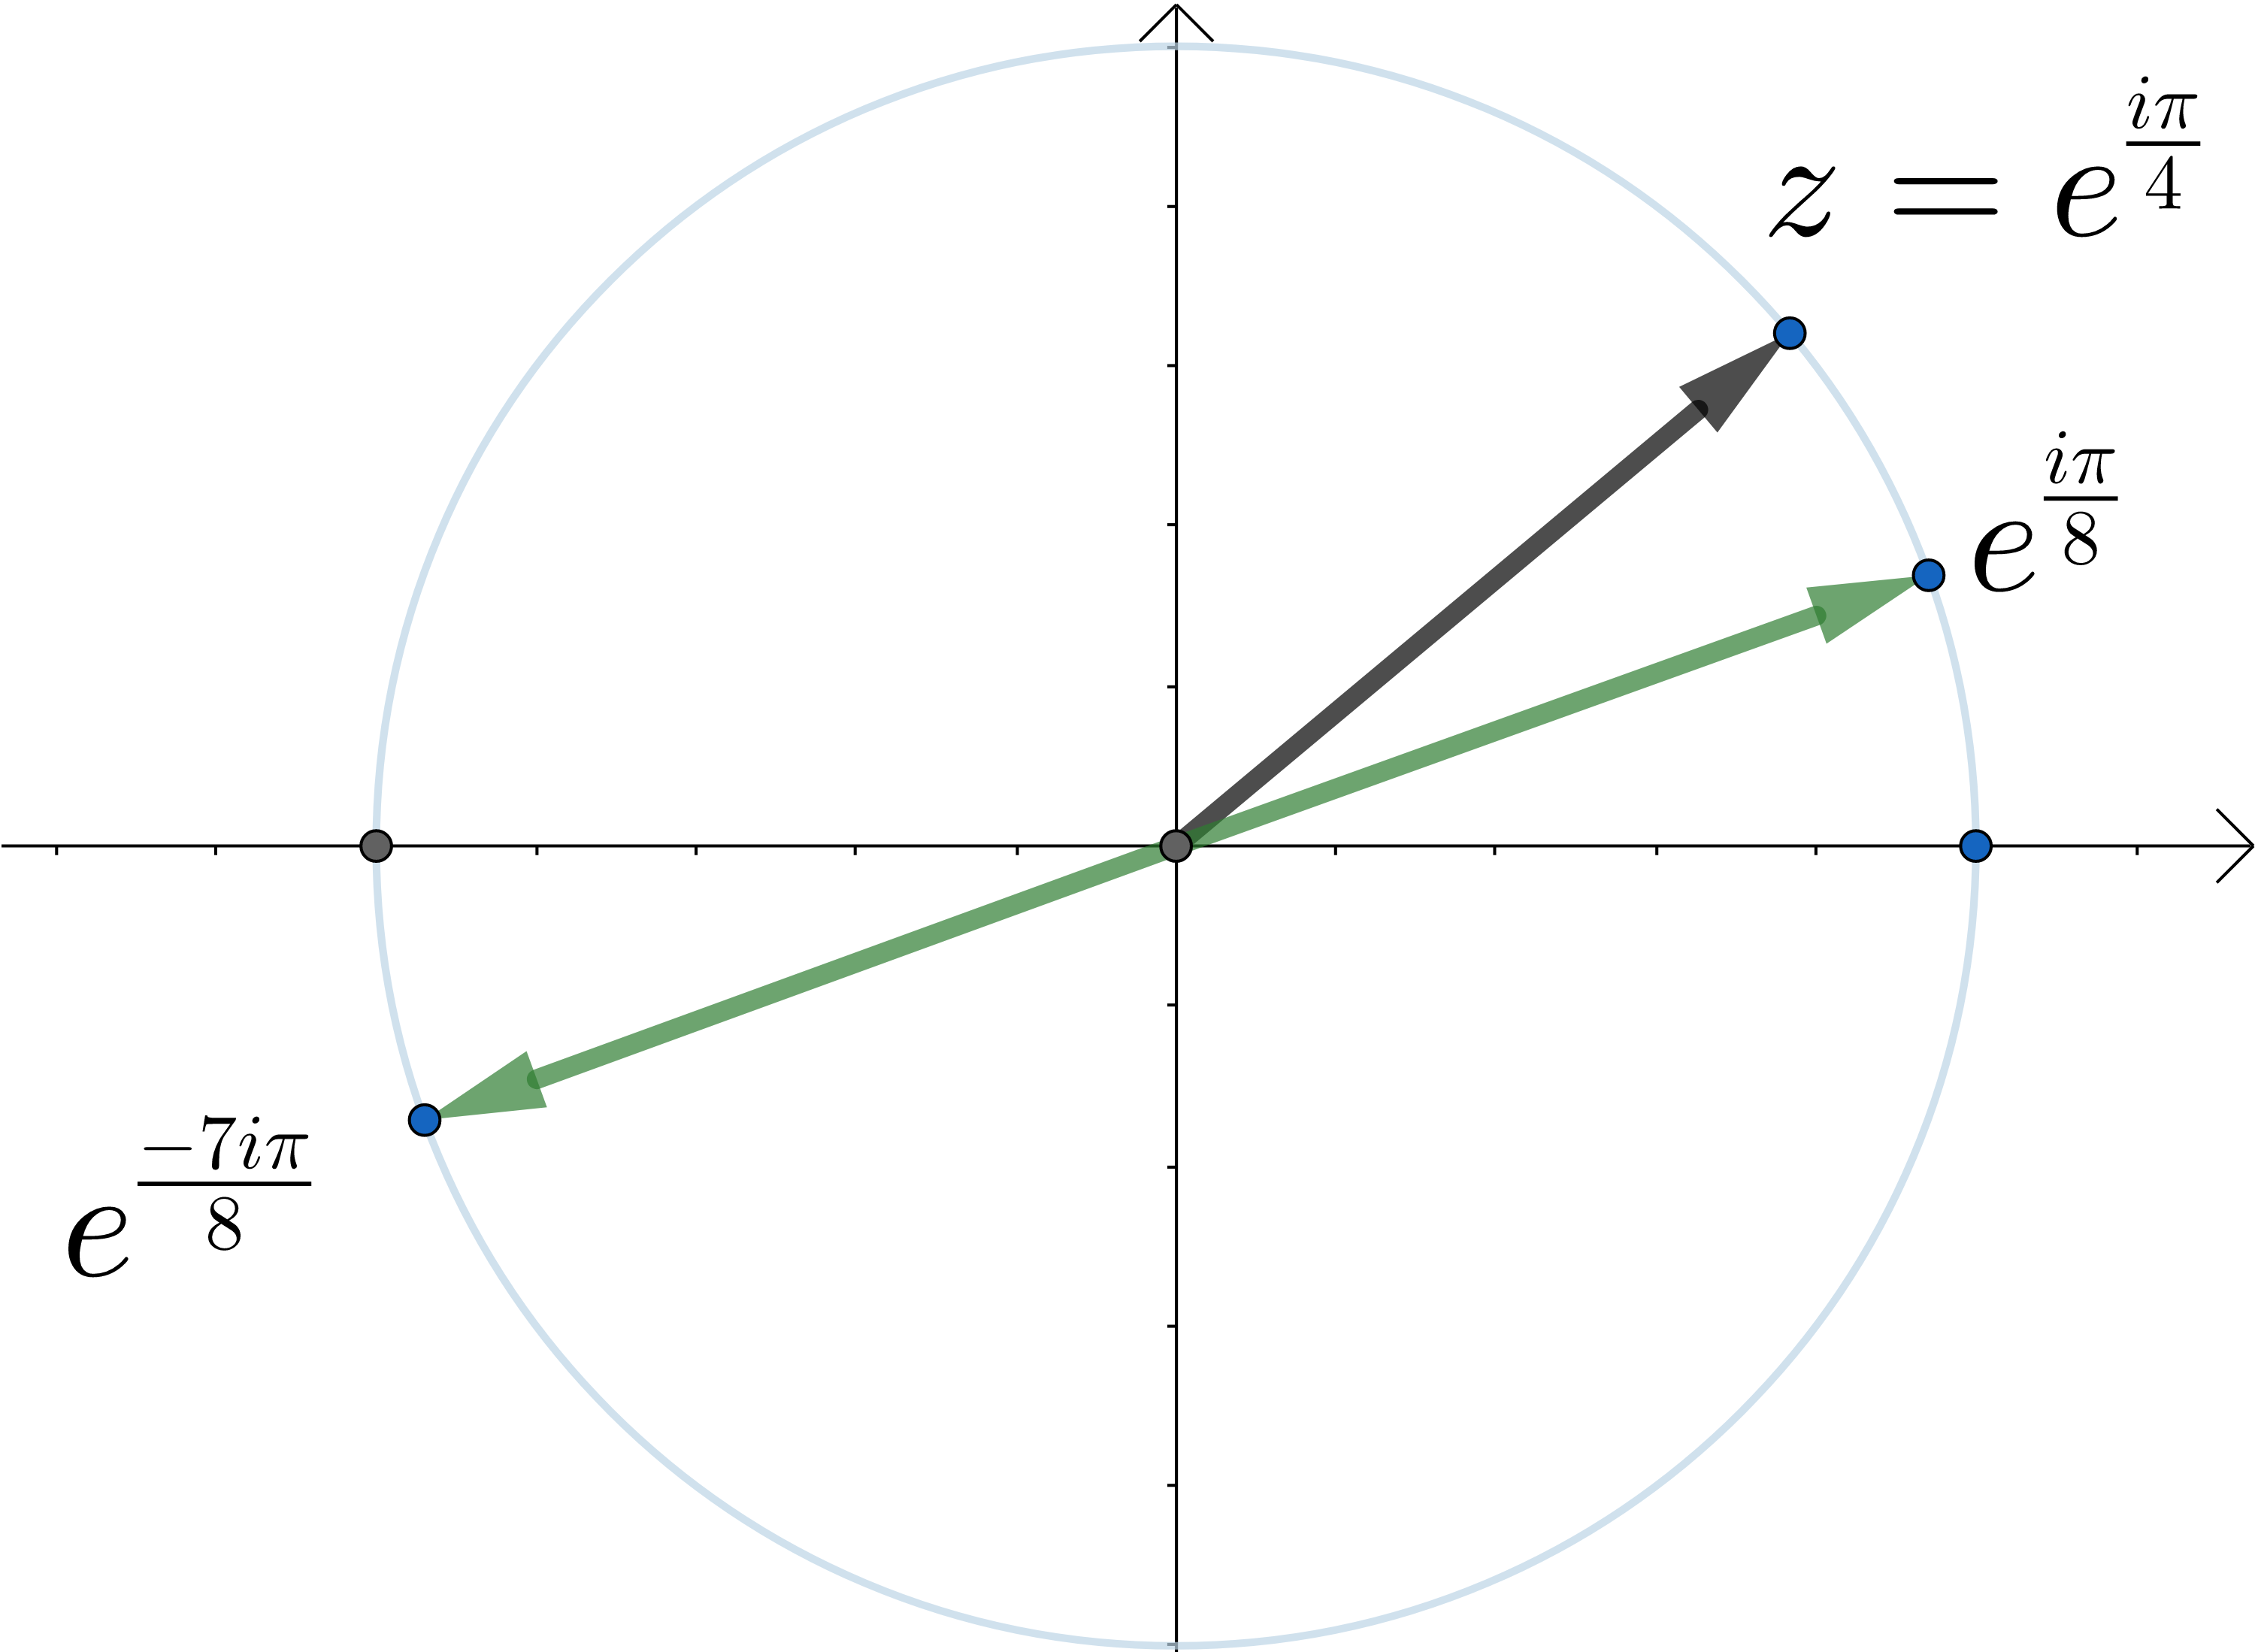
\includegraphics[scale=3]{roots-pi-4.png}
\end{frame}

\begin{frame}{N-th roots}
Similarly there is a principal $n$-th root:\vfill
{\LARGE
\begin{equation*}
\sqrt[n]{z} = \sqrt[n]{R\cdot e^{i\alpha}} = \sqrt[n]{R}\cdot e^{\frac{i\alpha}{n}}
\end{equation*}}\vfill
and all numbers of the form\vfill
{\LARGE
\begin{equation*}
	\sqrt[n]{R}e^{\frac{i\alpha+2ki\pi}{n}}
\end{equation*}
}\vfill
are also $n$-th roots of $z$ for $k\in \mathbb{N}$.
\end{frame}

\begin{frame}{Cube roots}
The cube roots of $8$ are $2$, $2e^{\frac{2i\pi}{3}}$ and $2e^{\frac{-2i\pi}{3}}$:\vfill
\begin{center}
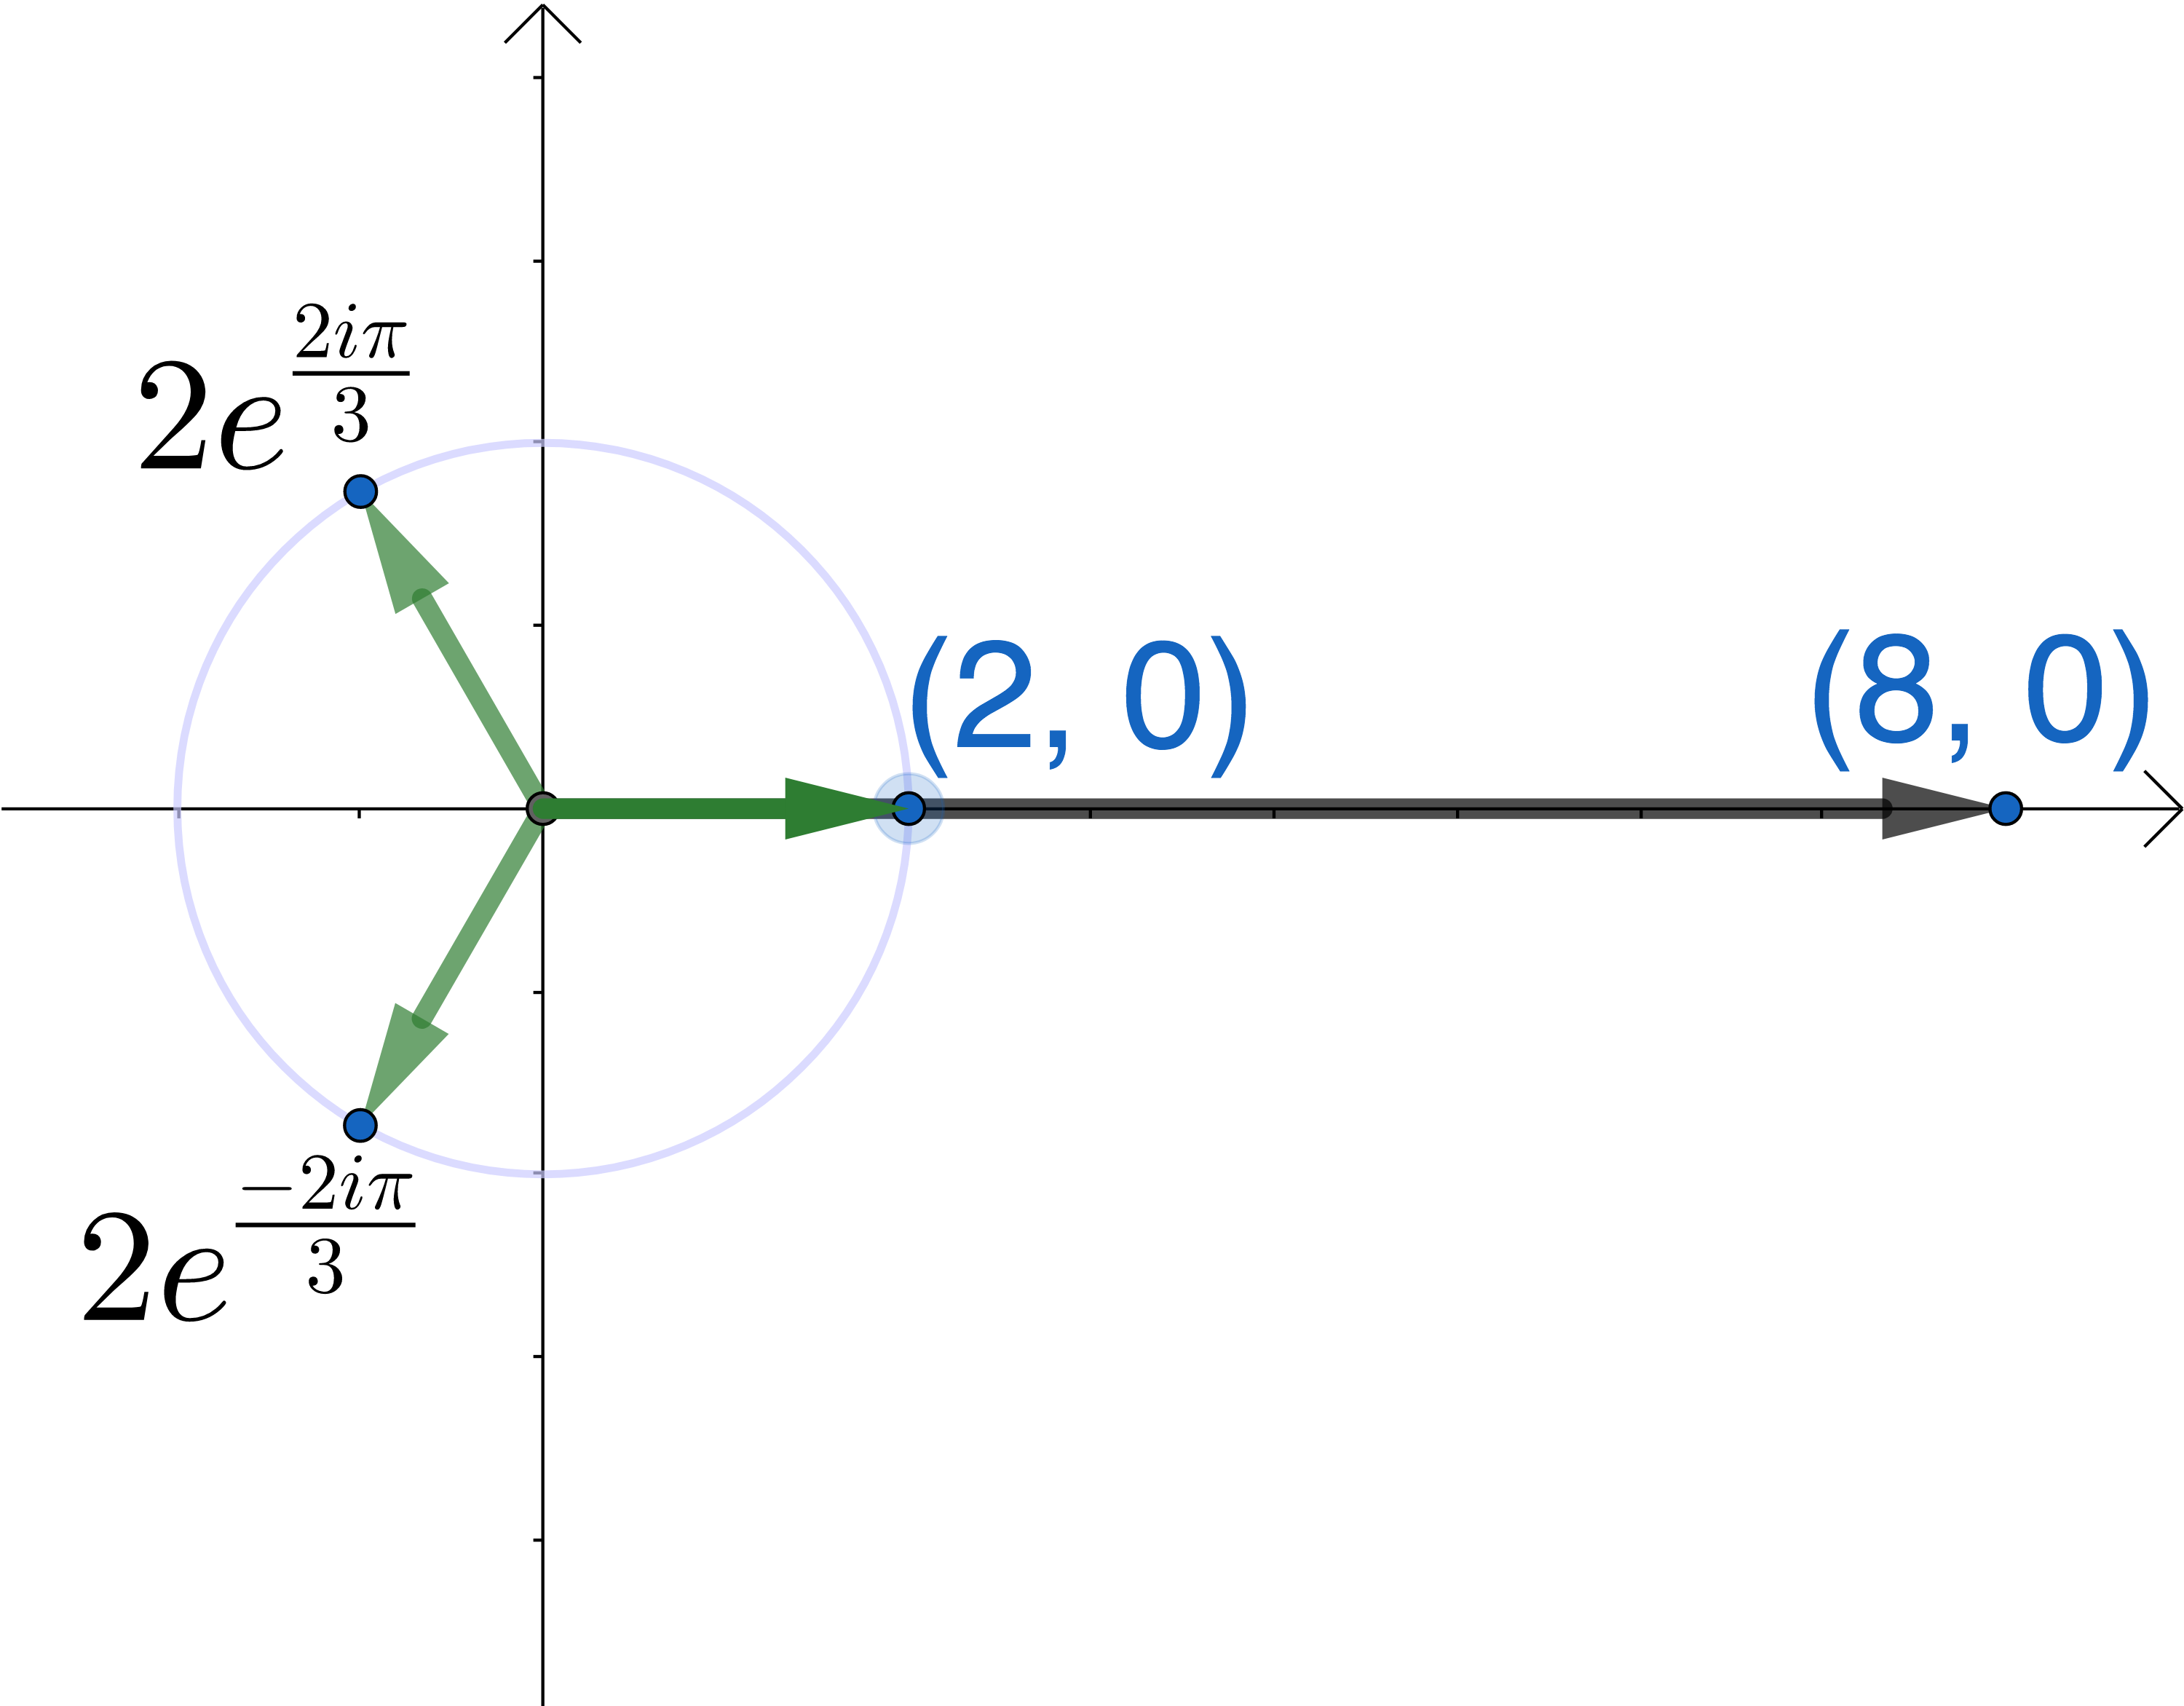
\includegraphics[scale=0.7]{cube-roots-8.png}
\end{center}
\end{frame}

\begin{frame}{Cube roots}
The cube roots of $i$ are $e^{\frac{i\pi}{6}}$, $-i$ and $e^{\frac{5i\pi}{6}}$:
\begin{center}
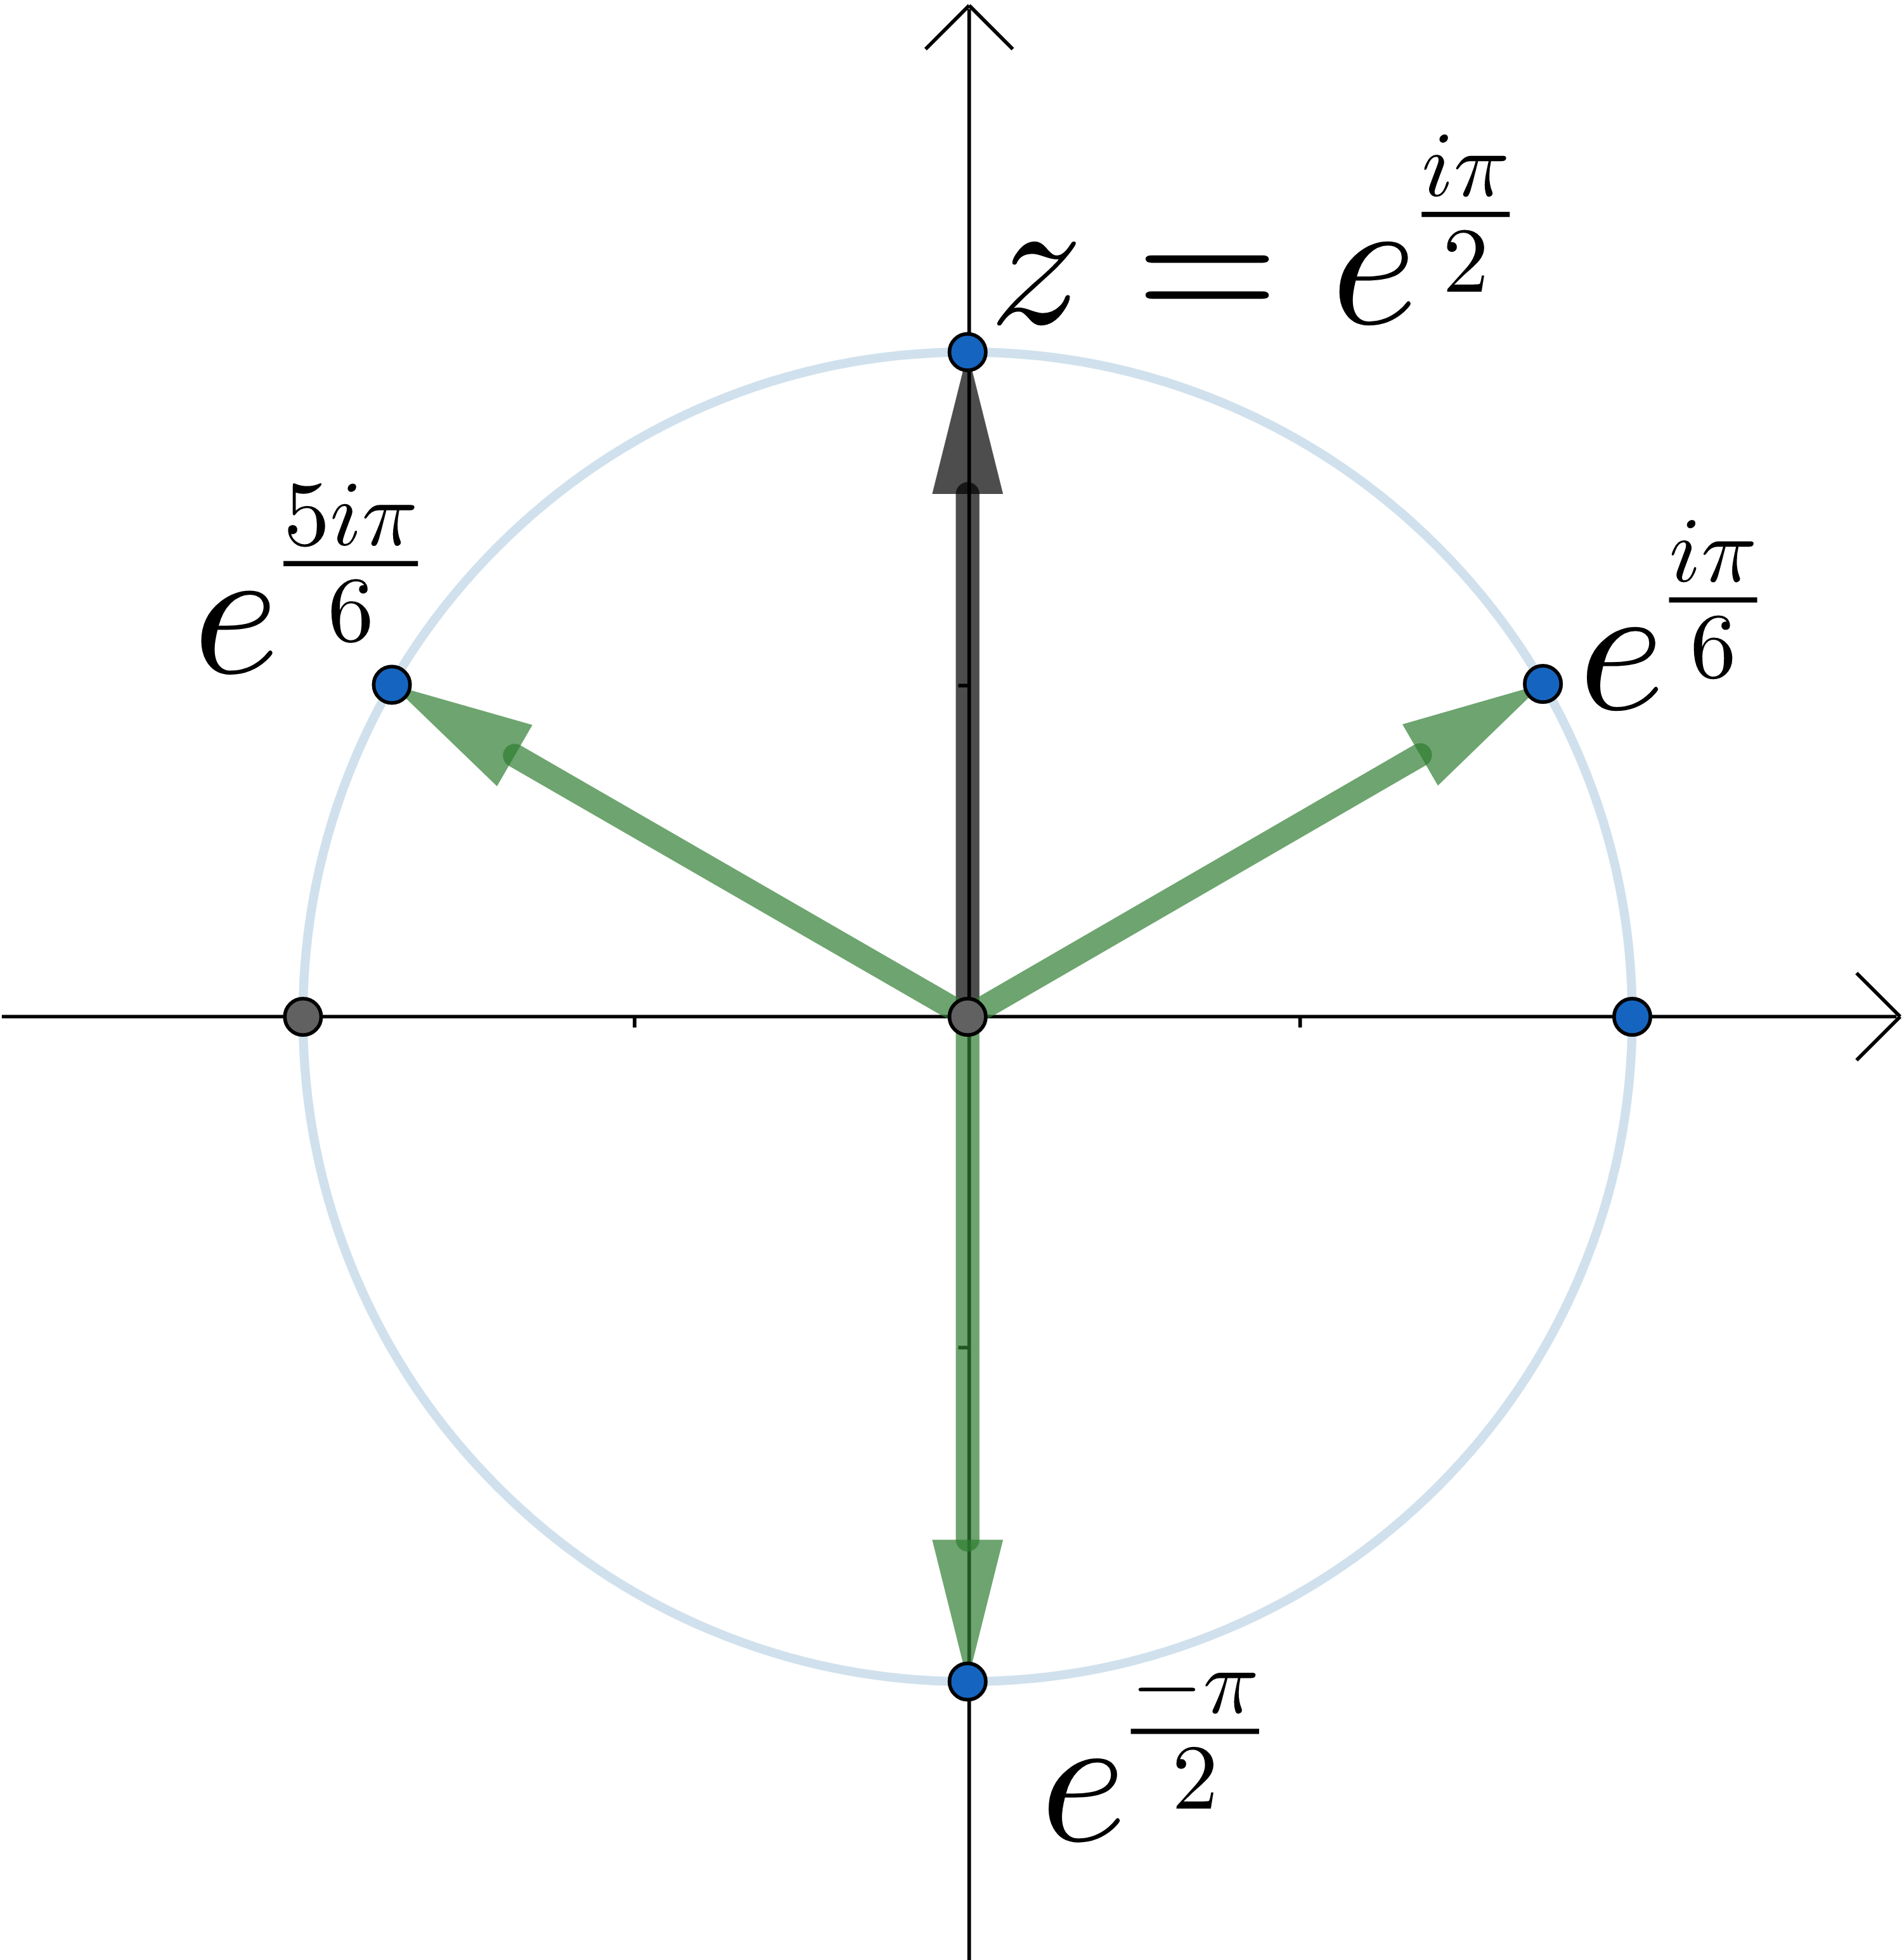
\includegraphics[scale=2]{cube-pi-2.png}
\end{center}
\end{frame}

\begin{frame}{4-th roots}
The fourth roots of unity are: $1$, $i$, $-1$ and $-i$:
\begin{center}
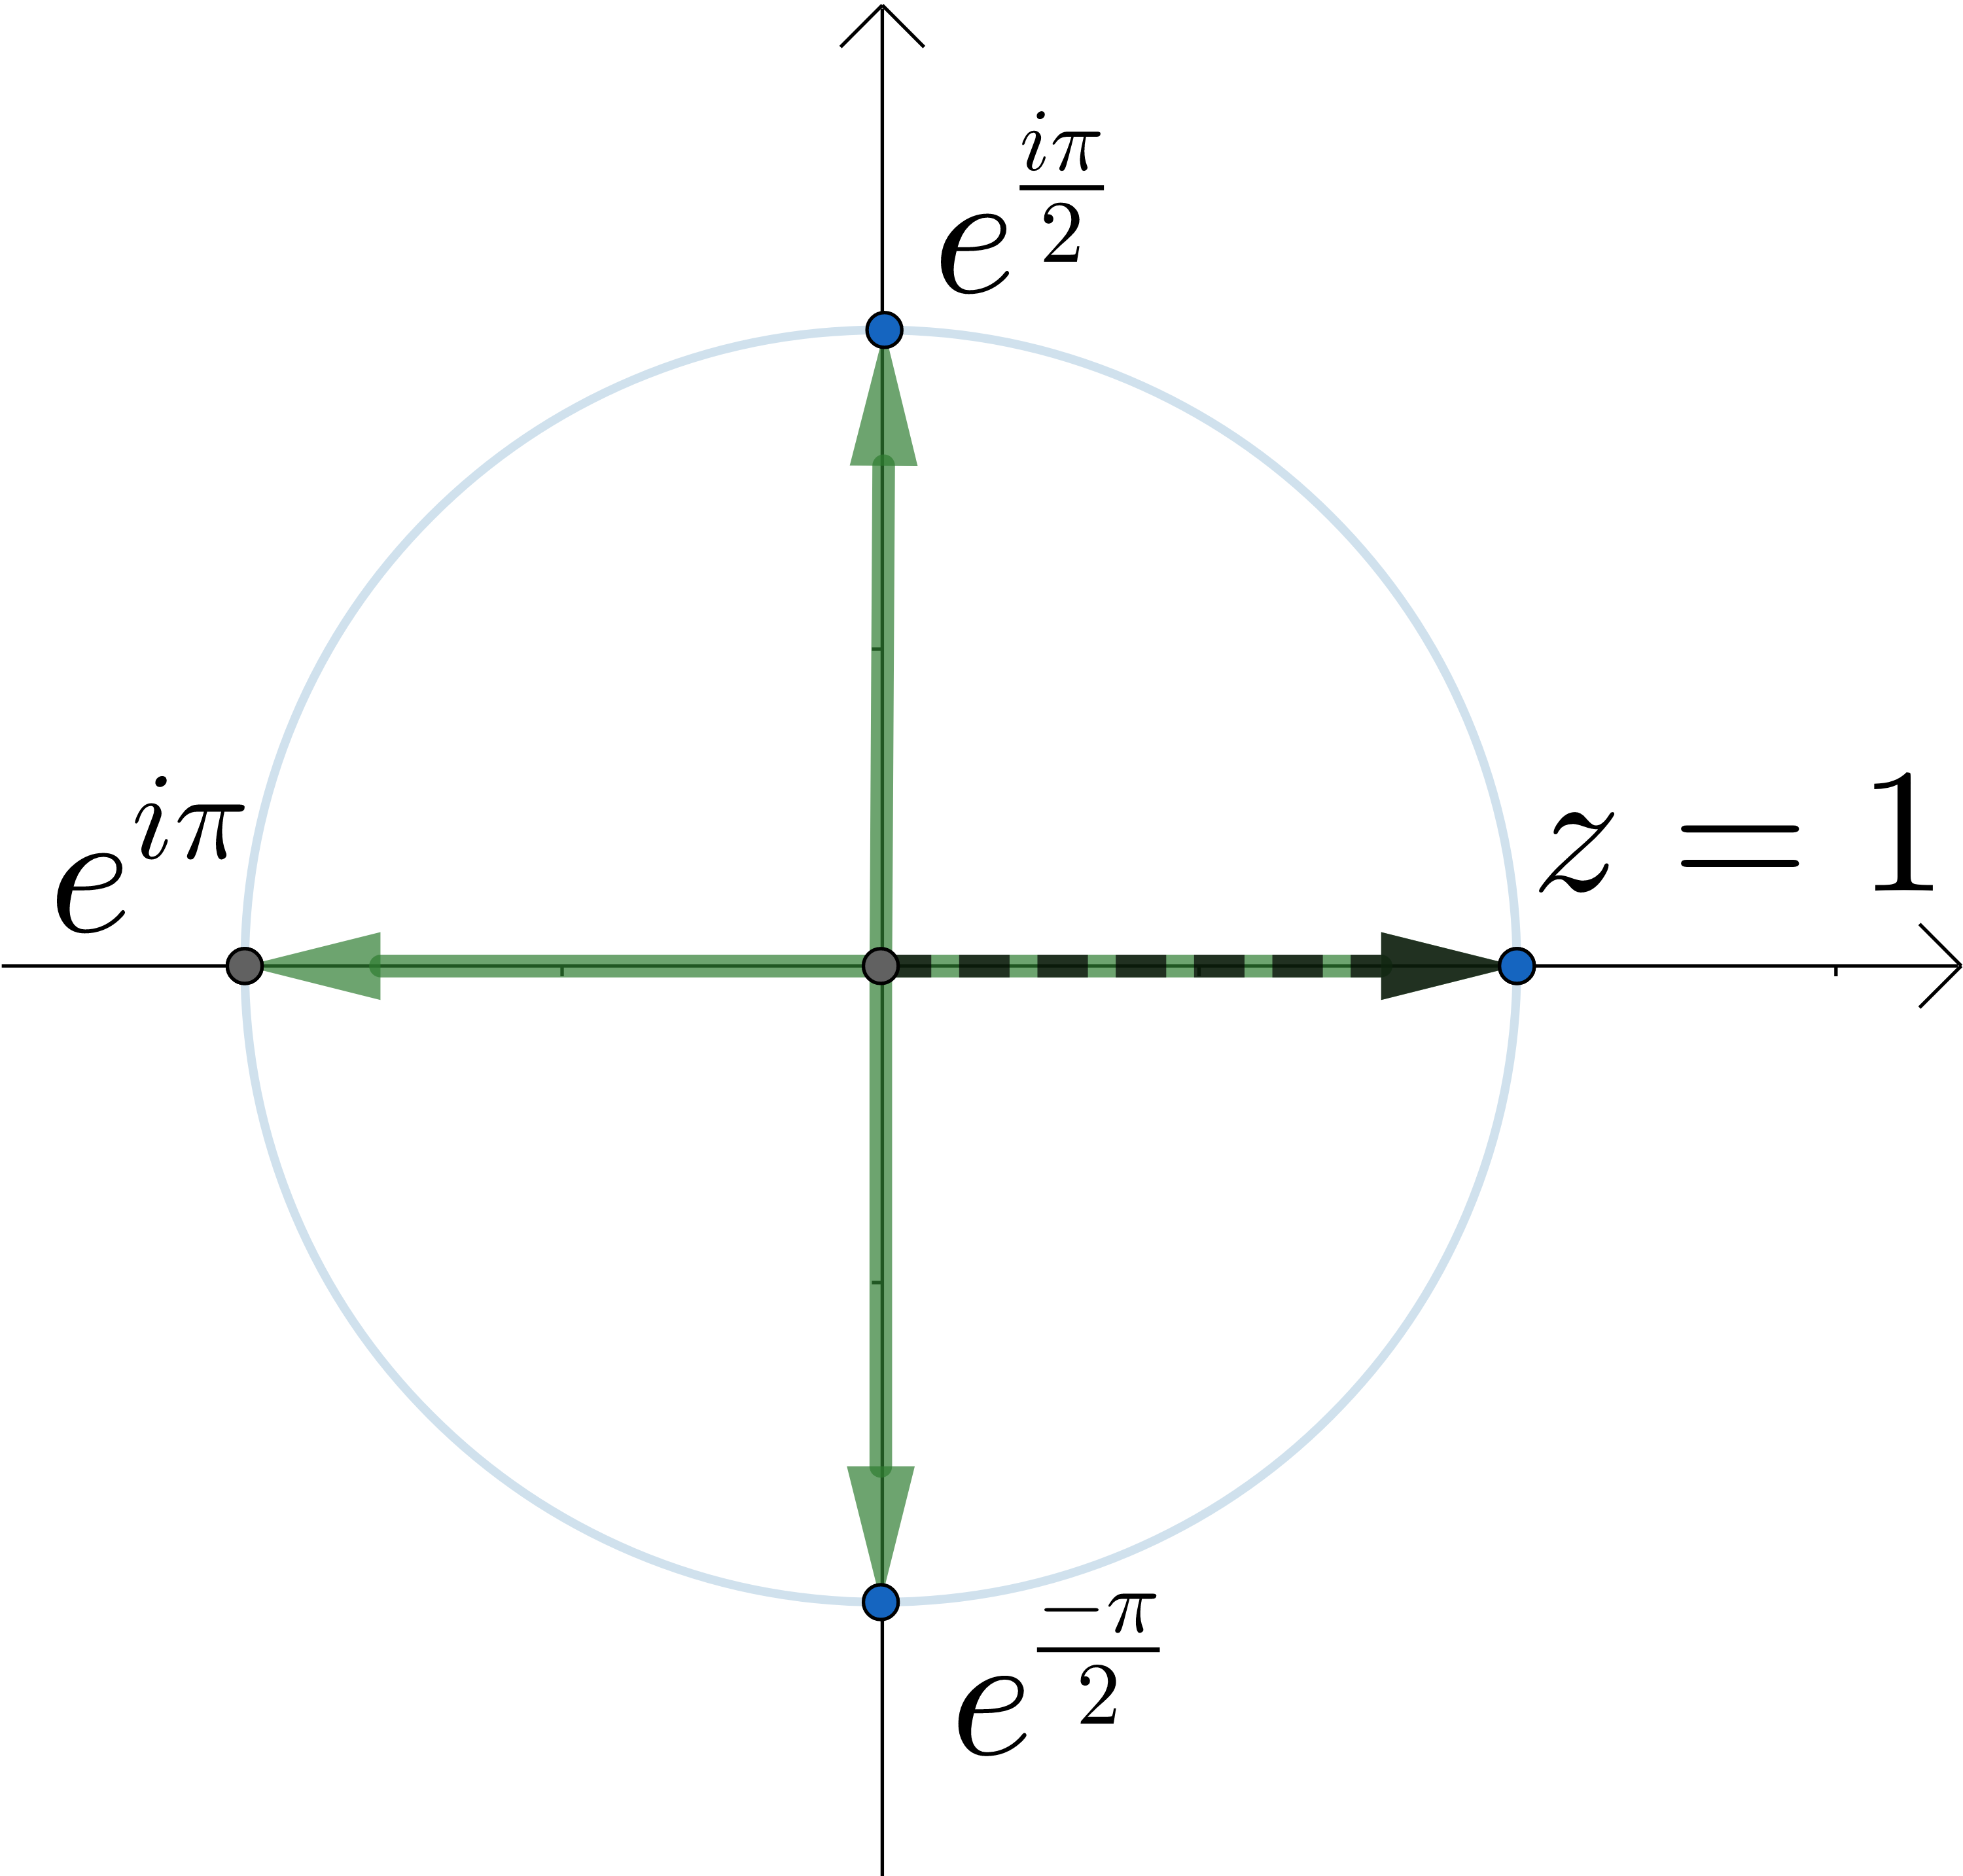
\includegraphics[scale=2]{four-roots-unity.png}
\end{center}
\end{frame}

\begin{frame}{Questions?}
Questions?
\end{frame}

\begin{frame}{Examples}
\begin{example}
Find all solutions to the following equations:
\begin{itemize}
	\item $z^2 = 25$. % ANS: -5 and +5
	\item Find all solutions to $z^2 = -1$ % ANS: i and -i
	\item Find all solutions to $z^2 = e^{\frac{i\pi}{4}}$ % ANS: e^{i*pi/8} and e^{-7*i*pi/8}
	\item Find all solutions to $z^3 = -1$.
	\item Find all solutions to $z^4 = 2(\sqrt{3}i-1)$. % ANS: sqrt{6}/2 + sqrt{2}/2i and + -sqrt{2}/2 +sqrt{6}/2 i and -sqrt{6}/2 - sqrt{2}/2i and  + sqrt{2}/2 -sqrt{6}/2 i
\end{itemize}
\end{example}
\begin{example}
Find all sixth roots of unity.
\end{example}
\end{frame}

\section{Quadratic formula}

\begin{frame}
\begin{beamercolorbox}[sep=12pt,center]{part title}
\usebeamerfont{section title}
\insertsection\par
\end{beamercolorbox}
\end{frame}

\begin{frame}{Quadratic formula}
If $a$, $b$ and $c$ are \emph{complex numbers} then the equation
\begin{equation*}
az^2+bz+c = 0
\end{equation*}
has two solutions given by
\begin{equation*}
	z_1 = \frac{-b+\sqrt{b^2-4ac}}{2a} z_2 = \frac{-b-\sqrt{b^2-4ac}}{2a}
\end{equation*}
\begin{itemize}
	\item We assume $a\neq 0$.
	\item The formula is unchanged $a$, $b$ and $c$ real numbers.
	\item We always get a solution.
\end{itemize}
\end{frame}

\begin{frame}{Galois theory for quadratics}
If $u$ and $v$ are the roots of $f(x) = z^2 + bz+c$ then
\begin{equation*}
(z-u)(z-v) = z^2 - (u+v)z + uv
\end{equation*}
and so
\begin{align*}
b & = -u-v\\
c & = uv
\end{align*}
\begin{itemize}
	\item If $f$ is a \emph{real} quadratic we need both $u+v$ and $uv$ to be real.
	\item This implies that $u = \overline{v}$ .
\end{itemize}
\end{frame}

\begin{frame}{Examples}
\begin{example}
Solve $z^2-14z+58 = 0$.
\end{example}
\begin{example}
Find a real quadratic with $5-2i$ as a root. What is the other root?
\end{example}
\begin{example}
Find a real quadratic with $-3+4i$ as a root. What is the other root?
\end{example}
\end{frame}

\begin{frame}
\begin{example}
Find the roots of $z^2-3iz+(-3+i) = 0$.
\end{example}
\begin{example}
Verify that $4-i$ is a root of $z^2 - (2-3i)-(10+6i) = 0$. Find the other root.
\end{example}
\begin{example}
Solve $z^2-(3-2i)z + (5-i) = 0$.
\end{example}
\end{frame}

\end{document}